\chapter{The LEF File: Physical Abstraction of Cells and Layers}

\begin{tldr}
\begin{itemize}[leftmargin=*,nosep]
  \item \textbf{Last chapter:} the \texttt{.lib} stored cell behavior as NLDM lookup tables across PVT. \textbf{This chapter:} the LEF stores the same cell's physical footprint, so the placer can put it somewhere legal without ever opening the GDS.
  \item The \textbf{LEF (Library Exchange Format)} file gives the placer and router the \textbf{physical view} of every cell that the timing \texttt{.lib} characterized: bounding box, pin shapes, blockages, and which layer each pin lives on.
  \item LEF comes in two flavors that get shipped separately: a \textbf{technology LEF} (one per process node, describing metal layers, vias, and design rules) and a \textbf{cell LEF} (one per standard cell library, describing each \texttt{MACRO}).
  \item LEF deliberately throws away the transistor-level GDS. The placer never sees diffusion or poly. It sees rectangles on metal layers and a placement \texttt{SITE} grid. GDS only re-enters the flow at LVS and tape-out.
  \item Inside a \texttt{MACRO}: \texttt{SIZE} (width $\times$ height), \texttt{SYMMETRY}, \texttt{SITE}, one \texttt{PIN} block per logical pin (with \texttt{PORT} geometries on specific \texttt{LAYER}s), and \texttt{OBS} blockages that the router must avoid.
\end{itemize}
\end{tldr}

\section{Why the placer is blind to your beautiful layout}

Your standard cell layout is a stick diagram with diffusion, poly, contacts, and three or four metal layers. It is gorgeous. The placer does not care. When the placer drops an \texttt{INV\_X1} into a row, it is moving a small \textbf{rectangle of width $W$ and height $H$}, snapping its origin to a \texttt{SITE} on a row, and asking one question: \emph{do the pin shapes on M1 line up with a routing track?}

Everything else (the FET widths, the poly pitch, the well taps) is \textbf{stripped out} before the cell ever reaches P\&R. The file that does the stripping is the LEF.

\begin{figure}[h]
\centering
\begin{tikzpicture}[scale=1.0, every node/.style={font=\footnotesize}]
  % Cell boundary
  \draw[thick, fill=blue!3] (0,0) rectangle (6,4);
  % VDD rail (top)
  \draw[fill=red!30, draw=red!60!black] (0,3.7) rectangle (6,4.0);
  \node[red!60!black, font=\bfseries\footnotesize] at (3,3.85) {VDD rail (M1)};
  % VSS rail (bottom)
  \draw[fill=blue!30, draw=blue!60!black] (0,0) rectangle (6,0.3);
  \node[blue!60!black, font=\bfseries\footnotesize] at (3,0.15) {VSS rail (M1)};
  % Input pin A on M1
  \draw[fill=green!40, draw=green!50!black] (1.8,1.6) rectangle (2.4,2.4);
  \node[green!50!black] at (2.1,2.0) {\textbf{A}};
  % Output pin Y on M1
  \draw[fill=orange!40, draw=orange!60!black] (3.6,1.6) rectangle (4.2,2.4);
  \node[orange!60!black] at (3.9,2.0) {\textbf{Y}};
  % OBS region
  \draw[fill=gray!30, draw=gray!60!black, pattern=north east lines] (0.3,0.5) rectangle (1.4,3.5);
  \node[gray!50!black, font=\tiny] at (0.85,2.0) {\textbf{OBS}};
  % Routing tracks (dashed)
  \foreach \y in {0.6,1.2,1.8,2.4,3.0,3.6} {
    \draw[dashed, gray!50, very thin] (0,\y) -- (6,\y);
  }
  % Cell height bracket
  \draw[<->, thick] (-0.5,0) -- (-0.5,4);
  \node[rotate=90, anchor=south] at (-0.7,2) {cell height = 6 tracks};
  % Width
  \draw[<->, thick] (0,-0.4) -- (6,-0.4);
  \node at (3,-0.7) {SIZE width (3 sites $\times$ site\_x)};
  % Origin marker
  \filldraw[red] (0,0) circle (1.5pt);
  \node[red, anchor=north west, font=\tiny] at (0.05,-0.05) {origin (0,0)};
\end{tikzpicture}
\caption{Abstract physical view of an \texttt{INV\_X1} as seen through the LEF. The placer sees this rectangle, the VDD/VSS rails, the M1 pin shapes for \texttt{A} and \texttt{Y}, and the \texttt{OBS} blockage. It never sees the transistors underneath.}
\label{fig:inv-abstract}
\end{figure}

\begin{hook}
\textbf{LEF is the placer's passport photo.} The cell's full GDS face stays home; only the \textbf{rectangle, the pins, and the rails} travel through P\&R. If the passport photo is wrong, the cell still gets stopped at the border (DRC).
\end{hook}

\begin{hook}
\textbf{Tech-LEF paints the streets; cell-LEF parks the cars.} The tech-LEF declares which metal layers exist, their pitch, and their direction. The cell-LEF tells the tool where each cell parks on those streets. Mismatched grids mean the cars do not fit between the curbs.
\end{hook}

\begin{gut}
A placer is dropping an \texttt{INV\_X1} into a row. Which of these does it read from the LEF, and which from the \texttt{.lib}? (a) cell delay vs.\ load, (b) cell width in microns, (c) pin \texttt{A} input capacitance, (d) which metal layer pin \texttt{A} sits on.
\gutans{LEF: (b) and (d). Timing \texttt{.lib}: (a) and (c). LEF is physical only. The .lib is electrical only. They share cell names so the tool can join the two views.}
\end{gut}

\begin{gut}
You open a cell LEF and see \texttt{SIZE 0.6 BY 1.2}. Where does the unit (microns vs.\ database units) come from?
\gutans{The technology LEF, via the \texttt{UNITS} section (typically \texttt{DATABASE MICRONS 1000} or similar). The cell LEF inherits the unit; it does not redeclare it.}
\end{gut}

\begin{pausebox}
So far: LEF abstracts the physical view, ships in two pieces (tech + cell), and intentionally hides the GDS. Next we nail down the one sentence that justifies everything else in this chapter.
\end{pausebox}

\begin{keyidea}
The LEF is the \textbf{contract between the cell library and the placer/router}: it promises that a cell will occupy exactly this footprint, expose pins on exactly these layers at exactly these coordinates, and block routing in exactly these regions, so the tool can resolve placement and routing \textbf{without ever opening the GDS}.
\end{keyidea}

\section{Anatomy of a MACRO block}

A cell LEF is a stack of \texttt{MACRO} blocks. Each block declares the cell name, its bounding box, what kind of cell it is (\texttt{CLASS CORE}, \texttt{PAD}, \texttt{BLOCK}, etc.), which placement site it snaps to, and then one \texttt{PIN} sub-block per logical pin plus an \texttt{OBS} sub-block for blockages.

\begin{figure}[h]
\centering
\begin{lstlisting}[style=eda, basicstyle=\ttfamily\footnotesize, frame=single]
MACRO INV_X1
  CLASS CORE ;
  ORIGIN 0 0 ;
  SIZE 0.6 BY 1.2 ;
  SYMMETRY X Y ;
  SITE CoreSite ;

  PIN A
    DIRECTION INPUT ;
    USE SIGNAL ;
    ANTENNAGATEAREA 0.14 ;
    PORT
      LAYER M1 ;
        RECT 0.18 0.40 0.24 0.80 ;
    END
  END A

  PIN Y
    DIRECTION OUTPUT ;
    USE SIGNAL ;
    PORT
      LAYER M1 ;
        RECT 0.36 0.40 0.42 0.80 ;
    END
  END Y

  PIN VDD
    DIRECTION INOUT ; USE POWER ;
    PORT LAYER M1 ; RECT 0.00 1.13 0.60 1.20 ; END
  END VDD

  PIN VSS
    DIRECTION INOUT ; USE GROUND ;
    PORT LAYER M1 ; RECT 0.00 0.00 0.60 0.07 ; END
  END VSS

  OBS
    LAYER M1 ; RECT 0.05 0.10 0.14 1.10 ;
  END
END INV_X1
\end{lstlisting}
\caption{A cell-LEF \texttt{MACRO} excerpt for an \texttt{INV\_X1}. Coordinates are in microns (set by the tech LEF). Pins \texttt{A} and \texttt{Y} expose M1 rectangles; \texttt{VDD}/\texttt{VSS} stripe the top and bottom; \texttt{OBS} blocks a region of M1 from the router.}
\label{fig:lef-listing}
\end{figure}

A few items deserve a closer look. \texttt{SYMMETRY X Y} tells the placer it may mirror this cell about either axis (commonly used to flip every other row so VDD/VSS rails abut). \texttt{SITE CoreSite} ties the cell to a placement site defined in the tech-LEF; the cell's width must be an integer multiple of the site width. \texttt{OBS} is a router-only directive that says \emph{do not route here}, typically used to hide internal M1 jumpers from the routing tool.

\section{Worked example: site arithmetic for an INV\_X1}

\move{1}
Given: cell \texttt{SIZE 0.6 BY 1.2} (microns). Tech-LEF declares \texttt{SITE CoreSite SIZE 0.2 BY 1.2}. We want: how many sites the cell occupies horizontally, its area, and whether it aligns to the row grid.


\move{2}
Sites occupied horizontally: $N_{\text{sites}} = \dfrac{W_{\text{cell}}}{W_{\text{site}}} = \dfrac{0.6}{0.2} = 3$ sites. The cell consumes a contiguous run of \textbf{three placement sites}.


\move{3}
Row alignment: row height is the site height $= 1.2\,\si{\micro\meter}$, and the cell height is also $1.2\,\si{\micro\meter}$. Match. The cell fits exactly in one row, with its VDD pin on the top edge and VSS on the bottom.


\move{4}
Cell area: $A = W \times H = 0.6 \times 1.2 = 0.72\,\si{\micro\meter\squared}$. This is what the placer reports for utilization accounting, not the active silicon area.


\move{5}
Sanity check: if a designer had written \texttt{SIZE 0.55 BY 1.2}, then $0.55 / 0.2 = 2.75$ sites. The placer would either reject the macro at library load (\emph{cell width not a multiple of site width}) or silently round up to 3 sites, wasting $0.05\,\si{\micro\meter}$ of width per instance. Multiply that by half a million instances and you have lost a chunk of die area to a bad library.


\move{6}
Conclusion: a healthy library always reports \texttt{SIZE} widths that are exact integer multiples of the \texttt{SITE} width, and the cell's row height equals the row pitch. \textbf{Both equalities are silently assumed by the placer.}


\begin{figure}[h]
\centering
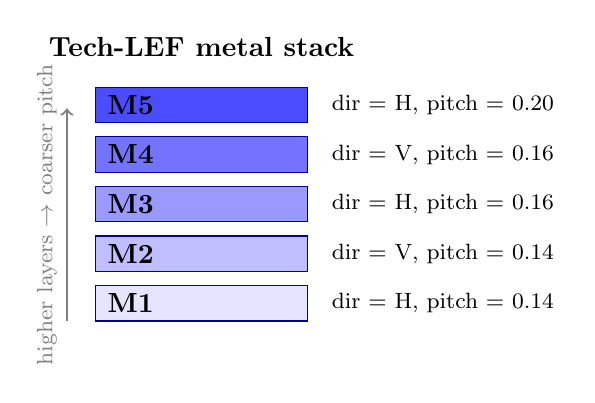
\begin{tikzpicture}[scale=0.9, every node/.style={font=\footnotesize}]
  % Layer stack
  \foreach \y/\name/\dir/\pitch in {0/M1/H/0.14, 1/M2/V/0.14, 2/M3/H/0.16, 3/M4/V/0.16, 4/M5/H/0.20} {
    \draw[fill=blue!\the\numexpr10+15*\y\relax, draw=blue!60!black] (0,\y*0.7) rectangle (3,\y*0.7+0.5);
    \node[black, font=\bfseries] at (0.5,\y*0.7+0.25) {\name};
    \node[anchor=west] at (3.2,\y*0.7+0.25) {dir = \dir, pitch = \pitch\,\si{\micro\meter}};
  }
  \node[anchor=south, font=\bfseries] at (1.5,3.6) {Tech-LEF metal stack};
  % Arrow indicating up
  \draw[->, thick, gray] (-0.4,0) -- (-0.4,3.0) node[midway, left, rotate=90, anchor=south] {higher layers $\to$ coarser pitch};
\end{tikzpicture}
\caption{A simplified tech-LEF view of the metal stack. Each \texttt{LAYER} declaration carries a \texttt{DIRECTION} (horizontal or vertical preferred routing) and a \texttt{PITCH}. The router uses these to lay tracks; the cell-LEF places its pin \texttt{RECT}s so they land on those tracks.}
\label{fig:metal-stack}
\end{figure}

\begin{pitfall}
\textbf{Four ways a LEF will silently wreck your block:}
\begin{itemize}[leftmargin=*,nosep]
  \item \textbf{Tech-LEF vs.\ cell-LEF confusion.} Loading two tech-LEFs (e.g., one from the foundry and one from the IP vendor) causes contradictory \texttt{LAYER} definitions. The tool may pick the wrong one without warning.
  \item \textbf{M1 pin access at advanced nodes.} At 7nm and below, M1 is so dense that a pin \texttt{RECT} may have zero legal access points after considering via rules. The router fails to connect it, even though DRC on the cell alone passes.
  \item \textbf{OBS misuse.} An overly aggressive \texttt{OBS} on M2 forces all routes to detour, blowing up congestion. Too little \texttt{OBS} and the router crosses an internal node, creating shorts at LVS.
  \item \textbf{Mismatched \texttt{SITE} definitions.} The std cell library was characterized on \texttt{SITE CoreSite} ($0.2 \times 1.2$), but the floorplan rows were generated on a slightly different site. Cells will not snap, and the tool emits thousands of placement-legality errors.
\end{itemize}
\end{pitfall}

\begin{sidebar}
\textbf{Tech-LEF vs.\ cell-LEF, and where LEF came from.} The \textbf{tech-LEF} is shipped by the foundry (or PDK provider) once per process node. It declares units, the metal stack (layer names, directions, pitches, min width, spacing), via definitions, and the placement \texttt{SITE} grid. The \textbf{cell-LEF} is shipped per standard cell library and contains one \texttt{MACRO} per cell. Both files are plain ASCII, historically defined by \textbf{Cadence} in the late 1980s as an open interchange format paired with \textbf{DEF} (Design Exchange Format) for post-placement data. The pair (LEF/DEF) is still the lingua franca that lets a Synopsys placer eat a TSMC library or a Cadence router eat a Samsung library without binary glue.
\end{sidebar}

\begin{pdnote}
\begin{itemize}[leftmargin=*,nosep]
  \item \textbf{Arm PD intern.} When a new tech drop lands, the first thing you do is diff the tech-LEF against the previous version: layer pitches, via rules, \texttt{SITE} sizes. A silent pitch change forces a full re-floorplan.
  \item \textbf{Generic PD engineer.} If a block has unroutable nets concentrated around one cell type, open that cell's LEF and inspect its M1 pin \texttt{RECT}s and \texttt{OBS} regions. Pin-access problems are visible at the library level long before they explode in the router log.
  \item \textbf{VLSI interview.} Expect the question: \emph{What is in a LEF file, and how is it different from a GDS?} The crisp answer is: LEF is the \textbf{abstract physical view} (bounding box, pins, blockages, on metal layers only) used by P\&R; GDS is the \textbf{full polygon-level layout} used only at LVS and tape-out.
\end{itemize}
\end{pdnote}

\begin{checkpoint}
You should now be able to: (1) state what LEF abstracts away and why, (2) name the two LEF flavors and what each contains, (3) read a \texttt{MACRO} block and identify \texttt{SIZE}, \texttt{SITE}, \texttt{PIN}, \texttt{PORT}, \texttt{LAYER}, \texttt{OBS}, (4) compute site occupancy for a given cell width.

\mnemonic{\textbf{``SIZE the cell, SITE the row, PIN the layer, OBS the rest.''} Four verbs map one-to-one onto the four LEF keywords the placer/router actually consults on every cell.}
\end{checkpoint}
